\documentclass{article}
\usepackage[margin=1.5cm,bottom=2cm]{geometry}
\usepackage{fancyhdr}
\usepackage{graphicx}
\usepackage[section]{placeins}
\pagestyle{fancy}

\begin{document}
\fancyhead[L]{ 
\includegraphics[width=2cm]{au_logo.png} }
\fancyhead[R]{PHYS 2250: General Physics II}
\fancyfoot[C]{\thepage}
\vspace*{0cm}
\begin{center}
	{\LARGE \textbf{Lab 2}}\\
	\vspace{.25cm}
	{\Large Vectors}
	%\vspace{0.25cm}
	%{\Large Due: Friday, September 4}
\end{center}

\section*{Overview}
In this lab you will practice adding vectors together and then check your results by balancing several force vectors. 

\section*{Setup}
This procedure for this lab is straightforward. On your lab bench you will find masses and a so-called ``vector table''. You will suspend masses from a hanger which is attached to a ring at the center of the table. A pulley will redirect the gravitational force acting on the mass to pull on the ring, exerting a force on it. You will randomly choose the values for mass and angle for two of the hanging masses, and then calculate the net force of these two forces. You will check your result using the vector table. As we will soon discuss in class, the magnitude of gravitational force which acts on a mass $m$ is given by:
\begin{equation}
|\vec{F}|=mg
\end{equation}
Where $g$ is a constant having the approximate value $g=9.81$m/s$^2$.
Here is a step-by-step procedure:

\begin{enumerate}
	\item Choose a mass and attach it to the hanger
	\item Hang the hanger at an angle of your choosing
	\item Record the information in row $\vec{F}_1$ of table \ref{tab} (record the magnitude of the force, the angle as recorded on the vector table, and the x and y components, assuming that $0^\circ$ points in the positive x direction.)
	\item Pick a mass and different angle for your second mass, and record the information in row $\vec{F}_2$.
	\item Add the two vectors together to get the third vector, $\vec{F}_{sum}$.
	\item Now you will experimentally test your result for $\vec{F}_{sum}$. If the sum of $\vec{F}_1$ and $\vec{F}_2$ truly is $\vec{F}_{sum}$, then the force can be balanced by adding a third force to your vector table, with the same magnitude as $\vec{F}_{sum}$ but pointing in the opposite direction. This is illustrated in figure \ref{fig1}. Enter this force, called $\vec{F}_{balance}$ into the corresponding row of the table.
	\item If your calculations are correct, the net force on the ring should now be zero, and the ring will not move when you pull the pin. If the ring is not balanced, your calculation has gone wrong somewhere. Repeat the calculation until the ring balances.
	\item Now repeat the entire process, starting from step 1, twice more (using different values for mass and angle).
	
\end{enumerate}

\begin{table}
	\centering
	\begin{tabular}{|c|c|c|c|}
		\hline
		& $|\vec{F}|$&$\theta$&$<x,y>$\\
		\hline
		$\vec{F_1}$ & & & \\
		\hline
		$\vec{F_2}$& & & \\
		\hline
		$\vec{F}_\mathrm{sum}$ & & & \\
		\hline
		$\vec{F}_\mathrm{balance}$ & & & \\
		\hline 
	\end{tabular}
	\caption{An example data table}
	\label{tab}
\end{table}
\begin{figure}
	\centering
	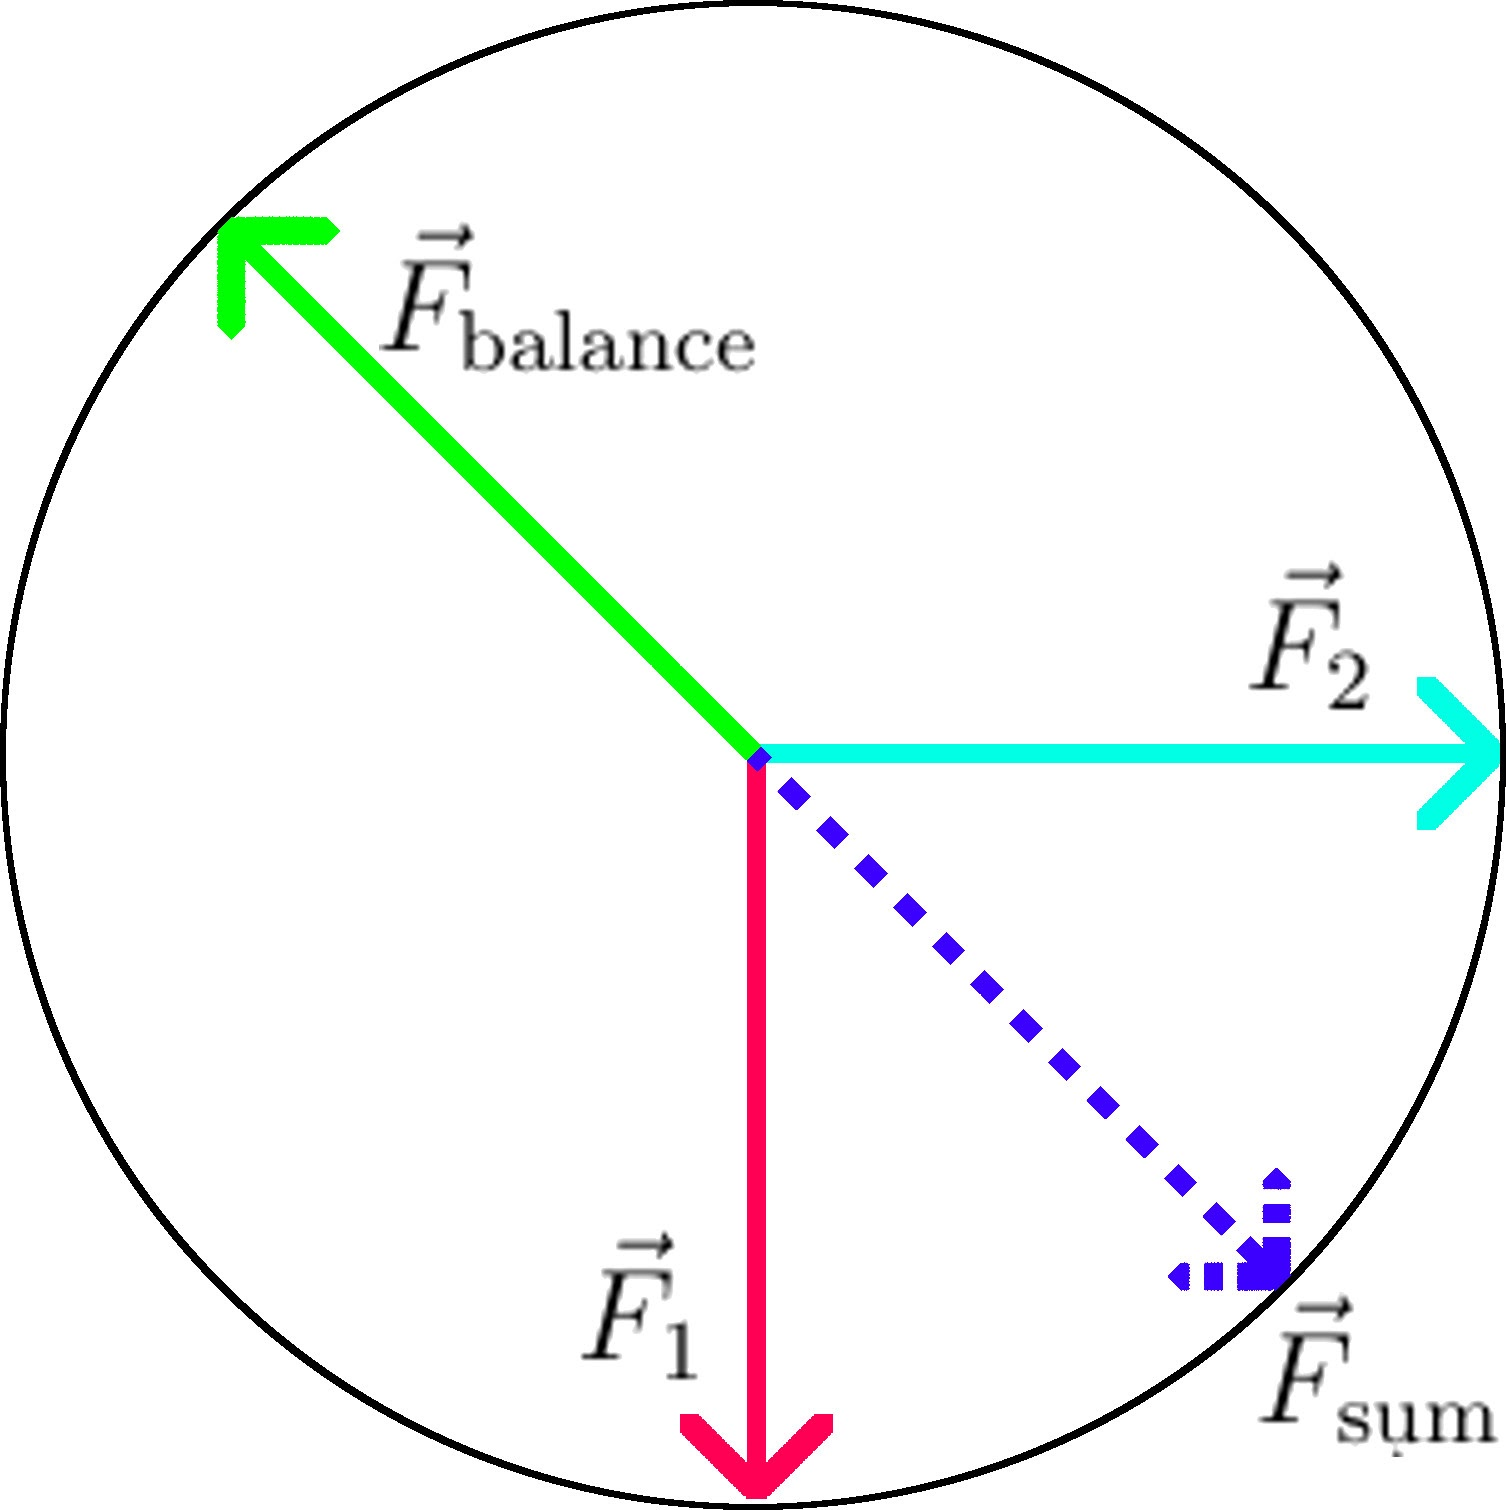
\includegraphics[width=0.3\textwidth]{diagram.jpg}
	\caption{}
	\label{fig1}
\end{figure}

\section*{Questions}
\begin{enumerate}
	\item Were you able to balance your forces (were your calculations correct)? Why or why not?
\end{enumerate}
\end{document}